
\chapter{Technical choice}



\section{Application created for test}

As it was explain before, I have to protect a specific application. To do my tests, and prove the concept of my
work, I choose to create a simple application. I plan to add some security issue to be more realistic.~\\


This application have three states, and two part. Firstly, there is an admin interface which contain the state
admin. This interface is connected on the port 9000. Only one specific known computer can access to this interface.
Of course, the aim of attackers is to arrive in this state.

Then there is the main application. It is connected to the port 9124, and everybody can connect to it. There is two
state ping and pong. If the application is in the state ping and the user send <<topong>> the application go to state
pong, and if the application is in the state pong and the user send <<toping>> the application go to the state ping.
There is also an unknown backdoor, if the user is in the state ping for the third time and he send <<admin>>, the
application go to the admin interface.

The figure \ref{fig:appli} represent a model of our application.


\begin{figure}[!h]
  \centering
  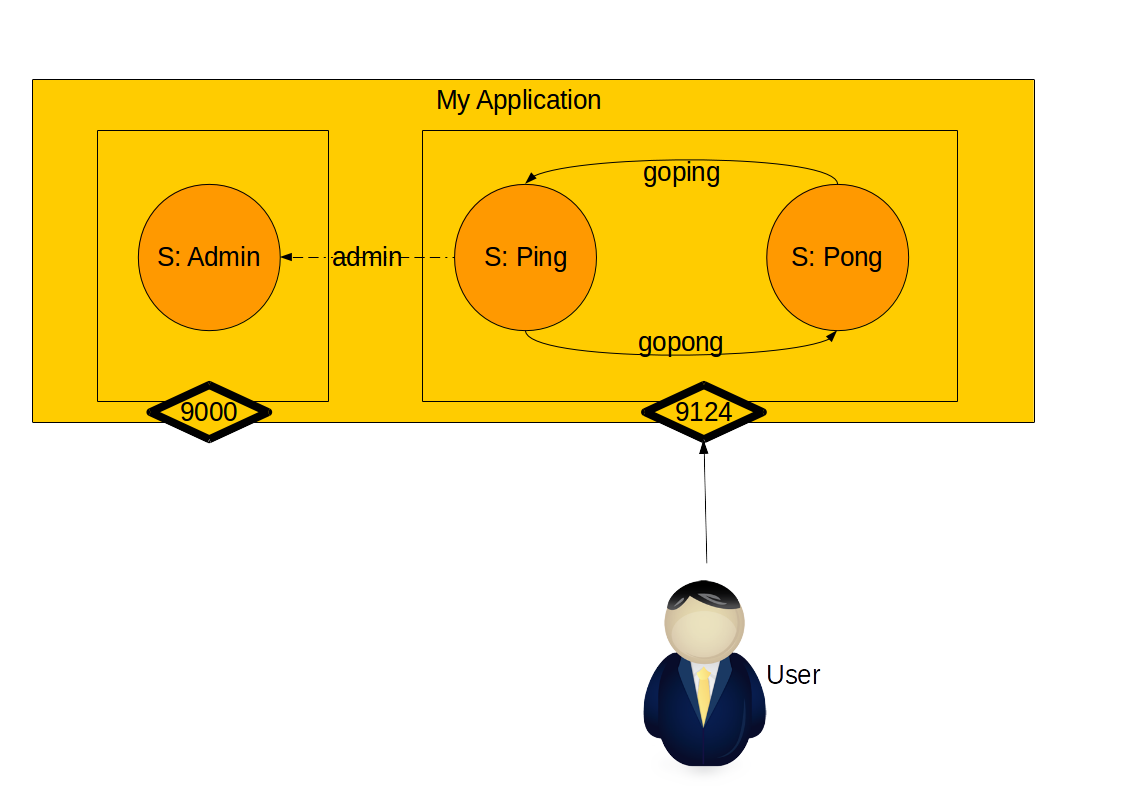
\includegraphics[width=0.9\textwidth]{appli}
  \caption{Model of the application}
  \label{fig:appli}
\end{figure}

\section{IDS}

Choice of SELKS

\section{SIEM}

Implement my SIEM



%%% Local Variables:
%%% mode: latex
%%% TeX-master: "../rapport_de_base"
%%% End:
